\begin{figure*}[!h]
    \centering
    \begin{subfigure}[b]{0.24\textwidth}
        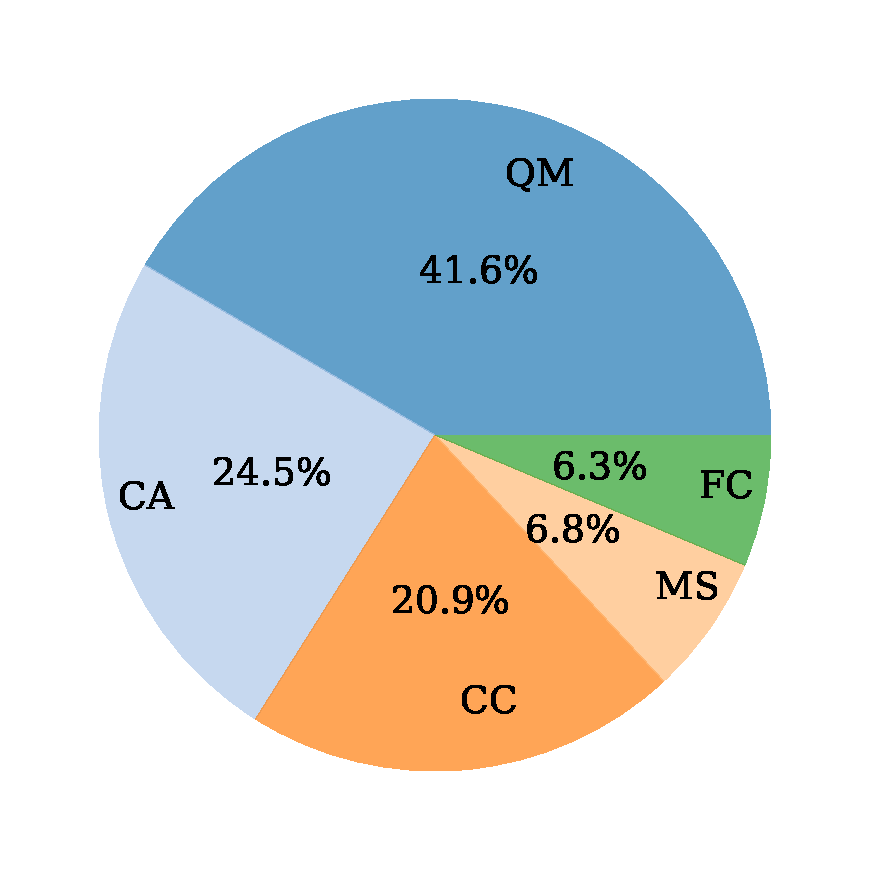
\includegraphics[width=\linewidth]{figure/pdf/error-type_pie_chart_llama_gsm8k.pdf}
    \caption{LLaMA3-8B}
    \label{fig:error_type_llama}
    \end{subfigure}
    \hfill
    \begin{subfigure}[b]{0.24\textwidth}
        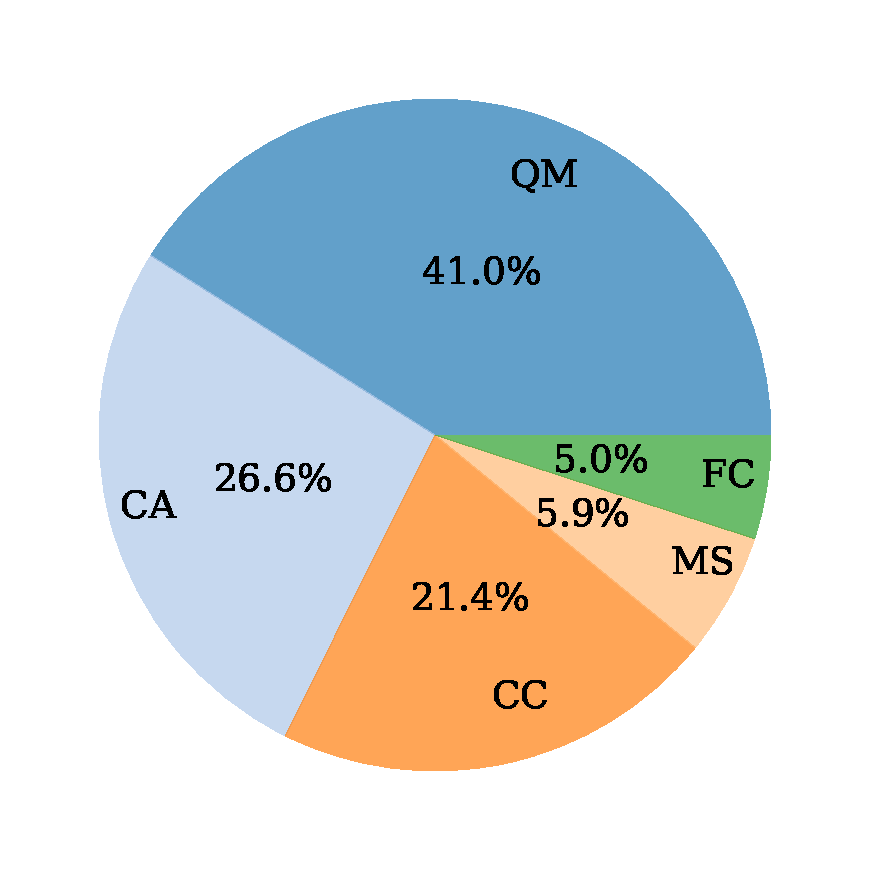
\includegraphics[width=\linewidth]{figure/pdf/error-type_pie_chart_mistral_gsm8k.pdf}
        \caption{Mistral-7B}
        \label{fig:error_type_mistral}
    \end{subfigure}
    \hfill
    \begin{subfigure}[b]{0.24\textwidth}
        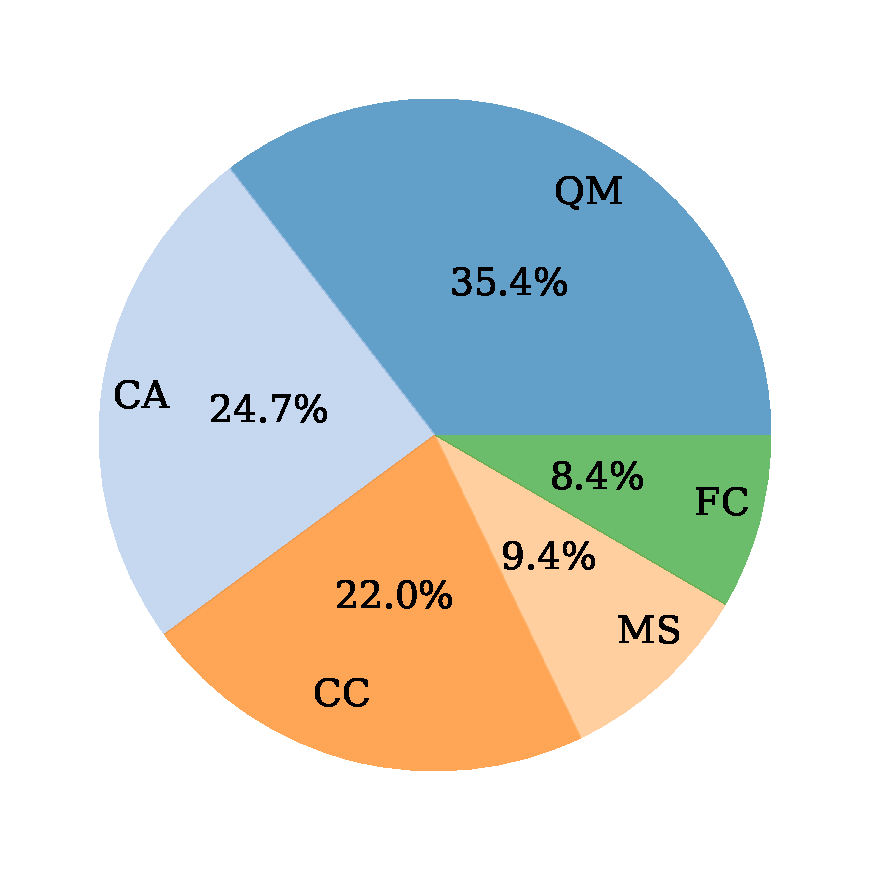
\includegraphics[width=\linewidth]{figure/pdf/error-type_pie_chart_deepseek_gsm8k.pdf}
        \caption{DeepSeekMath-7B}
        \label{fig:error_type_deepseek}
    \end{subfigure}
    \hfill
    \begin{subfigure}[b]{0.24\textwidth}
        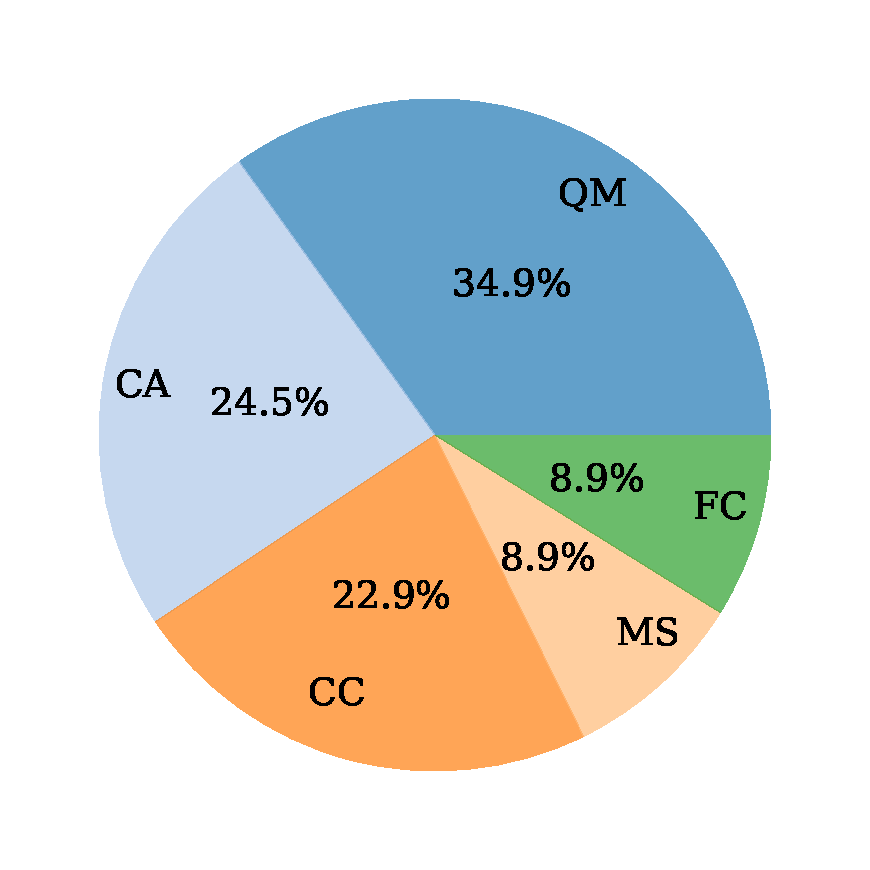
\includegraphics[width=\linewidth]{figure/pdf/error-type_pie_chart_qwen_gsm8k.pdf}
        \caption{Qwen2-Math-7B}
        \label{fig:error_type_qwen}
    \end{subfigure}
    \caption{Error type distribution of the different models on the GSM8K test set, with \textit{GPT-4o} as the error classification model. Error types that account for less than 1\% are omitted to avoid text overlap.}
    \label{fig:error_type_gsm8k}
\end{figure*}
